\documentclass{article}
\usepackage{emnlp2021}
\usepackage{times}
\usepackage{latexsym}
\usepackage[utf8]{inputenc}
\usepackage[T5]{fontenc}\usepackage{amsfonts}
\usepackage{microtype}
\usepackage{tabularx}
\usepackage{graphicx}
\usepackage{appendix}

\graphicspath{ {./images/} }

\title{Điện toán nhận thức: \\
Một bản tóm tắt và những thách thức trong nghiên cứu}

\author{
J. Octavio Gutierrez-Garcia\\
Instituto Tecnológico Autónomo de México \\
octavio.gutierrez@itam.mx
\And 
Emmanuel López-Neri \\
Universidad del Valle de México \\
emmanuel.lopezne@uvmnet.edu
}
\begin{document}
\maketitle

\begin{abstract}

Điện toán nhận thức là một lĩnh vực nghiên cứu đa ngành hướng đến việc xây dựng mô hình tính toán và cơ chế đưa ra quyết định dựa trên quá trình sinh học của bộ não, khoa học nhận thức và tâm lý học.
Mục tiêu của việc xây dựng mô hình điện toán nhận thức là cho phép hệ thống máy tính khả năng hiểu biết biết, suy nghĩ và cảm nhận.
Đóng góp chính trong bài báo này bao gồm
(i) đưa ra cái nhìn sâu sắc về hệ thống tính toán bằng việc liệt kê mô tả các định nghĩa của nó, các lĩnh vực tương tự, các thuật ngữ.
(ii) phân loại những nghiên cứu hiện tại về điện toán nhận thức theo mục tiêu nghiên cứu
(iii) trình bày đánh giá ngắn gọn về những cách tiếp cận điện toán nhận thức
(iv) nhận diện những vấn đề mở trong nghiên cứu lĩnh vực điện toán nhận thức

Các từ khóa \textit{cognitive computing; computational intelligence; artificial intelligence;}

\end{abstract}

\section{Giới thiệu} \label{sec:1-introduction}
Nhận thức là một quá trình của tư duy trong việc tạo ra kiến thức \citet{vaughn2012feeling} và sự hiểu biết bằng việc thu nạp mô tả trừu tượng về thế giới.
Tuy nhiên, chú ý rằng ko có một khái niệm được chấp nhận rộng rãi về định nghĩa của nhận thức hoặc của tư duy, mặc dù có những nghiên cứu rất rộng về nhận thức của con người.
Do đó điện toán nhận thức (cognitive computing - đưa ra bởi \citet{valiant1995cognitive} ) đã được định nghĩa theo những cách khác nhau bởi những nhà nghiên cứu, tùy thuộc vào thời gian và bối cảnh.

\Citet{valiant1995cognitive} định nghĩa điện toán nhận thức như là một quy tắc kết nối những thần kinh học, nhận thức tâm lý và trí tuệ nhân tạo lại với nhau.

\Citet{brasil2001hybrid} phát biểu rằng điện toán nhận thức là những công nghệ nổi bật, lấy cảm hứng quá trình sinh học để xử lý thông tin bên trong hệ thần kinh, lập luận của con người, đưa ra quyết định và chọn lọc tự nhiên. Tuy nhiên, chú ý rằng chọn lọc tự nhiên, định nghĩa bởi \Citet{hancock2008detecting}, là quá trình mà những đặc tính mong muốn được truyền từ nhóm chiếm ưu thế vượt lên trên những đặc tính không mong muốn theo thời gian, định nghĩa này thì rất khác với định nghĩa về nhận thức trong quá trình tư duy để tạo ra kiến thức.

\Citet{preissl2012compass} mô tả điện toán nhận thức như là "đi tìm một hàm gần giống cho tư duy, sử dụng năng lượng thấp, dung tích nhỏ, thực hiện trong thời gian thực của não người.

\Citet{szymanski2000satisfaction} cho rằng điện toán nhận thức là một lĩnh vực nổi bật của việc thăm dò tin tức dựa trên những quy tắc từ hành vi, nhận thức, máy tính và những khoa học liên quan.

\Citet{wang2006informatics} định nghĩa điện toán nhận thức là một thuật ngữ của nhận thức thông tin, là một lĩnh vực đa ngành áp dụng cách não bộ xử lý thông tin và đưa ra quyết định lên khoa học thông tin. Theo đó, \Citet{wang2006cognitive} định nghĩa điện toán nhận thức là một mô hình nổi bật của những phương pháp và hệ thống tính toán thông minh và dựa trên nhận thức thông tin, triển khai trí tuệ máy tính bằng tự suy luận, khả năng bắt trước cơ chế của bộ não.

\Citet{modha2011cognitive} và các cộng sự mô tả điện toán nhận thức bằng việc phát biểu mục đích của điện toán nhận thức, phát triển một cơ chế có liên kết, hợp nhất và phổ biến lấy cảm hứng từ khả năng tư duy.

\Citet{nahamoo2014cognitive} định nghĩa điện toán nhận thức như là một mô hình tính toán mới rất nền tảng cho việc xử lý những vấn đề của thế giới, khai thác một lượng thông tin khổng lồ sử dụng hàng loạt các máy tính song song có thể tương tác với con người và các hệ thống nhận thức khác. \Citet{evans2013utilizing} và cộng sự phát biểu rằng điện toán nhận thức tập trung vào miêu tả và xử lý thông tin.

Những nhà nghiên cứu khác đã chọn việc phác thảo điện toán nhận thức bằng phát biểu nguyên lý chính của nó, như \Citet{clark2002new}, người phát biểu rằng trong điện toán nhận thức có những cách phù hợp để trừu tượng hóa một mức độ cao một hành vi cụ thể, để nói về mục tiêu, kế hoạch, ràng buộc và phương pháp.

Những đóng góp chính của bài nghiên cứu nào gồm
(i) đưa ra những thông tin về điện toán nhận thức bằng liệt kê và mô tả những định nghĩa, lĩnh vực liên quan và những thuật ngữ (phần I và II); (ii) phân loại những nghiên cứu hiện tại về điện toán nhận thức theo mục tiêu nghiên cứu (phần III); (iii) trình bày một nhận xét xúc tích về những cách tiếp cận điện toán nhận thức (phần III. A-C); (iv) nhận diện những vấn về mở trong nghiên cứu lĩnh vực điện toán nhận thức (phần IV). Cuối cùng phần V bao gồm một số kết luận.

\section{Điện toán nhận thức và những ý tưởng liên quan} \label{sec:2-related-concepts}

Dựa trên những định nghĩa khác nhau về điện toán nhận thức, những khái niệm có liên quan liên quan với điện toán nhận thức là: kiến thức, thần kinh học, nhận thức tâm lý, trí tuệ nhân tạo, khoa học hành vi, khoa học nhận thức, khoa học máy tính, quy trình sinh học, hệ thần kinh, tranh luận, ra quyết định, nhận thức thông tin, não người và tư duy, khai thác sự bùng nổ thông tin - dữ liệu lớn \citep{cuzzocrea2011analytics}.

Theo \Citet{thornton2003life}, trí tuệ nhân tạo và nhận thức tâm lý là những nhánh trong khoa học nhận thức.

Trí tuệ nhân tạo có liên quan tới việc lập luận và quy trình bên trong suy nghĩ để xây dựng nên hệ thống thông minh có thể
(i) hành động và/hoặc suy nghĩ giống như con người 
(ii) suy nghĩ hoặc/và hành động có lý trí \citep{brewka1996artificial}. 
Lập luận là một loạt những bước cho phép đạt được kết luận (ví dụ: kiến thức) từ một số nền móng ban đầu \citep{walton1990reasoning}. Kiến thức có thể được định nghĩa như là việc hiểu một chủ đề để đạt được qua việc học và/hoặc thực hành. Bigdata tập trung vào việc lấy được kiến thức từ một lượng dữ liệu khổng lồ \citep{rubinstein2012big}, có thể được sử dụng để hỗ trợ việc ra quyết định. Ra quyết định được định nghĩa như một tiến trình của đánh giá và lựa chọn, dựa trên những điều kiện cho trước, chọn ra cái tốt nhất trong tập hai hoặc nhiều hơn lựa chọn để đạt được mục tiêu \citep{ozcan2011comparative}.

Nhận thức tâm lý tìm hiểu cách mà não tiếp nhận và dịch những cảm gíac từ bên ngoài. Thần kinh học nghiên cứu cách mà những kết nối giữa não bộ ảnh hưởng lên hành vi của một cá nhân \citep{imam2012digital}. Hệ thần kinh, tạo nên từ những neuron, phần ứng với tác nhân vật lý (vd cảm giác bên ngoài) và trao đổi những tín hiệu điện hóa giữa những neuron để điều khiển phản ứng của cơ thể. Một quá trình sinh học là một quá trình hóa học mà trong đó một chuỗi những sự kiện \citep{saxena2006absolute} ở tầng phân tử phản ứng với nhau để đạt được một mục đích sinh học (vd, sự trao đổi chất) \citep{dennis2003david}

Theo \citet{dwore1981behavioral}, \citet{gintis2004towards}, khoa học hành vi bao gồm sinh học, xã hội học, nhân loại học và tâm lý học. Sinh học (khoa học nghiên cứu cơ thể và thế bào) liên quan sâu sắc tới tính toán nhận thức. Theo cách thức hoàn toàn tương tự, xã hội học, nhân loại học và tâm lý học nắm giữ mối quan hệ ở cấp độ cao với điện toán nhận thức do những ngành này tập trung vào nghiên cứu hành vi của con người như những cá nhân đơn lẻ hoặc như xã hội.

Một điểm đáng chú ý là bộ não và tư duy thường bao gồm trong định nghĩa của điện toán nhận thức (\citet{wang2012denotational} và \citet{modha2011cognitive}), hai khái niệm này cũng hay được sử dụng lẫn lộn. Tuy nhiên, tư duy và bộ não khác nhau. Tư duy liên hệ đến một tập những hoạt động cho phép con người cảm nhận, suy nghĩ và hiểu biết trong khi bộ não là một bộ phận của cơ thể cho phép con người những năng lực để cảm nhận, suy nghĩ và hiểu biết. Do đó, điện toán nhận thức nên tập trung vào việc bắt trước những cơ chế của bộ não cho phép hệ thống máy tính có năng lực cảm nhận, suy nghĩ và hiểu biết.

Kết luận lại, điện toán nhận thức là một lĩnh vực nghiên cứu đa ngành với mục tiêu xây dựng mô hình tính toán và ra cơ chế quyết định dựa trên những xử lý thần kinh của bộ não, khoa học nhận thức và tâm lý học để cho hệ thống máy tính những năng lực hiểu biết, suy nghĩ và cảm nhận. Thêm vào đó, chú ý rằng mô hình điện thoán nhận thức có thể được hỗ trợ big-data, ví dụ cơ chế trích xuất thông tin tri chức của IBM Watson.

\begin{figure}[h!]
\caption{Phân loại các lĩnh vực nghiên cứu về điện toán nhận thức}
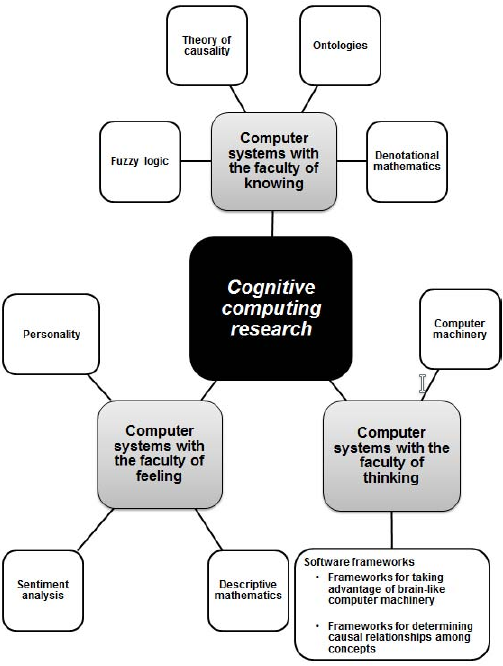
\includegraphics[width=\columnwidth]{fig-1-taxonamy}
\label{fig:1-taxonamy}
\end{figure}

\section{Những nghiên cứu hiện tại về điện toán nhận thức (2015)}\label{sec:3-current-researchs}

Trong khảo sát này, nhóm phân loại theo đối tượng của những nghiên cứu hiện tại về điện toán nhận thức ra thành những nhóm cung cấp (i) sự hiểu biết (ii) suy nghĩ và (iii) cảm nhận. Kết qủa tổng hợp như trong hình \ref{fig:1-taxonamy}, kết quả được phân tích trong phần A-C của phần III.


\subsection{Cho hệ thống máy tính khả năng hiểu biết}
Kết quả của nhận thức là kiến thức \citet{von1998cognition}, một vài nỗ lực nghiên cứu đã được thực hiện để định nghĩa một cách chính thức kiến thức từ góc nhìn của điện toán nhận thức.

\Citet{tian2011formal} công thức hóa kiến thức bằng việc tận dụng các ý tưởng đại số và xử lý số học thời gian thực. Khái niệm đại số là một framework tính toán được hỗ trợ bởi lý thuyết đối tượng-thuộc tính-quan hệ (object-attribute-relation) cho vận dụng kiến thức. Các khái niệm cơ bản có thể được định nghĩa, có quan hệ lẫn nhau, được so sánh và sắp xếp in thứ tự để tạo ra một mạng lưới của ý tưởng có thể công thức hóa được kiến thức. Xử lý đại số thời gian thực là hệ thống các ký hiệu toán học có khả năng mô tả kiến trúc hệ thống cũng như là hành vi tĩnh và động của các thành phần \citep{wang2002real}. Tian và nhóm kết hợp các ý tưởng đại số với xử lý đại số thời gian thực để đạt được khả năng thu thập và xử lý kiến thức.

Tương tự với Tian, \Citet{elbedwehy2014computational} và cộng sự cũng tận dụng xử lý đại số thời gian thực để thiết kế một mô hình nhận thức ngữ nghĩa của kiến thức, mô hình gồm 4 bước. Trong bước đầu tiên, một nguyên mẫu của kiến thức được tạo ra. Bước thứ hai gồm phân biệt giữa kiến thức liên quan và kiến thức không liên quan. Trong bước thứ ba, kiến thức được khái quát hóa và cuối cùng, bước thứ tư gồm việc phát triển một thuật toán được tạo ra từ một tập những quy tắc được thừa kế từ các bước trước. Như trong \Citet{elbedwehy2014computational}, \Citet{xiao2013knowledge} cũng nhấn mạnh việc cần giảm kiến thức, ví dụ như đạt đủ số lượng các thuộc tính để mô tả một đối tượng hoặc một ý tưởng thay vì đơn giản quy trình nhận thức.

\Citet{pena2012intelligent} mô hình hóa kiến thức bằng việc sử dụng lý luận nhân quả \citep{heckerman1995decision} và logic mờ (fuzzy) \citep{dunbar2007evolution}. Các ý tưởng và mối quan hệ giữa chúng được công thức hóa bằng bản thể luận. Tiếp đó những quan hệ nhân quả (thể hiện dưới đạng lập luận mờ) được định nghĩa cho các ý tưởng, ý tưởng thì được tích hợp vào một bản đồ nhận thức, ví dụ mô hình về nhận thức \citep{eden1992nature}. Bản đồ nhận thức thể hiện kết quả cuối cùng của mô hình nhận thức.

\citet{wang2012denotational}, \citet{wang2012inference} đề xuất một suy luận đại số, một biểu diễn toán học để định nghĩa một cách chính thức nhân quả và những loại khác trong suy luận, nó được định nghĩa bằng điều kiện, nguyên nhân, giá trị số, các sự kiện, theo thời gian, logic và suy luận logic mờ. Thêm vào đó, Wang cũng đề xuất một tập những toán tử để sửa logic suy luận biểu diễn kiến thức.

IBM Watson \cite{ferrucci2012introduction} sử dụng cách tiếp cận ngữ nghĩa, phương pháp mà IBM Watson đã dùng để vượt qua những người chơi xuất sắc nhất trong Jeopardy - một chương trình TV show kiểu hỏi-đáp. Hướng tiếp cận ngữ nghĩa của IBM bao gồm hơn 100 kĩ thuật xử lý ngôn ngữ tự nhiên [\citet{ferrucci2010building}, \citet{gliozzo2013semantic}], phần lớn trong này là cách tiếp cận xác suất. Để biểu diễn kiến thức, IBM Watson sử dụng cả cách tiếp cạn bán cấu trúc (ví dụ thuật ngữ) và có cấu trúc (bản thể luận). Tuy nhiên, thay vì trả lời các câu hỏi mở, IBM Watson tập trung vào cơ chế trích xuất kiến thức tự động. Cơ chế này có khả năng tiến hành phân tích từ vựng trên một lượng lớn các trang web. Kết quả phân tích là một tập các đối tượng (khái niệm/ý tưởng) và mối quan hệ giữ chúng.

\subsection{Cho hệ thống máy tính năng lực suy nghĩ}

Khi kiến thức đã được mô hình hóa, hệ thống điện toán nhận thức có thể tự giải quyết vấn đề bằng cách suy nghĩ về những mối quan hệ nguyên nhân kêt quả và những ý tưởng trong miền kiến thức đó. Theo hướng này, những nghiên cứu hướng đến việc cho hệ thống máy tính năng lực suy nghĩ nhắm đến mục tiêu 
(i) tầng thấp của hệ thống máy tính [ví dụ \citet{arthur2012building}, \citet{imam2012digital}, \citet{dunbar2007evolution}],
(ii) tầng cao của phần mềm [\citet{amir2013cognitive}, \citet{lawniczak2010computational}, \citet{wang2013cognitive}].

Máy móc có khả năng suy nghĩ. Phần cứng được thiết kế để có thể tái tạo lại bộ não con người

\citet{imam2012digital}, \citet{arthur2012building} đề xuất một phương pháp hướng sự kiện trên lõi xử lý thần kinh số, được tạo ra từ 256 neuron, 1024 sợi trục, 262144 khớp thần kinh (kết nối giữa 2 neuron). Có ba loại kết nối: kích động mạnh, kích động yếu và ức chế. Imam và cộng sự tranh luận rằng những con chip thần kinh đa hình (i) tương đối gọn, chiếm chỉ khoảng 4.2mm (ii) yêu cầu năng lượng tiêu thụ thấp, 45pJ mỗi spike citep{merolla2011digital}. Arthur và cộng sự chứng minh tạm thời rằng lõi xử lý thần kinh có thể cấu hình được (do số lượng lớn các kết nối giữa các neuron) bằng sử dụng 4 test cases: định hướng robot, phát triển một người chơi ảo cho pong, nhận diện số, và bộ nhớ kết hợp. Thêm vào đó, Esser và cộng sự \citep{esser2013cognitive} đã thiết kế và triển khai nhiều thuật toán khác tận dụng lợi thế của mạng lưới của nhân lõi thần kinh. Những thuật toán mới gồm cả nhận diện nhạc và phát hiện con mắt.

Cùng hướng này, \Citet{preissl2012compass} và cộng sự đề xuất Compass, một bộ xử lý đa luồng giả lập phương bắc địa lý - một con chip kĩ thuật số lấy cảm hứng từ bộ não với 4096 nhân thần kinh có khả năng đạt được hiệu nẵng mở rộng gần tối ưu. Kiến trúc nhận thức của Compass là sự kết hợp của số lượng neuron có thể so sánh được với não người. Thêm vào đó, Compass được cung cấp kèm với các giao tiếp sơ khai lý thuyết PGASS cho phép giao tiếp hiệu quả giữa các neuron.

Framework phần mềm cho phép suy nghĩ. Những tiến bộ trong phần mềm nhận thức cho phép suy nghĩ có thể được tập trung vào:

Tận dụng ưu thế của máy móc giống như bộ não, hoặc

Phát hiện mối quan hệ nhân quả giữa những ý tưởng của một miền kiến thức

Để tận dụng lợi thế của máy móc thiết kế giống như bộ não được đề xuất ở [\citet{arthur2012building},\citet{imam2012digital}, \citet{merolla2011digital}] \citet{amir2013cognitive} đã thiết kế một ngôn ngữ lập trình cho TrueNorth \citep{merolla2014million}. Nhóm tranh luận rằng kiến trúc phần cứng bắt chước não người được tạo ra từ một tập những tế bào thần kinh được kết nối yêu cầu một cách tiếp cận lập trình khác để thực thi các nhiệm vụ một cách hiệu quả. Từ đây thì Amir và nhóm đã nghĩ ra một ngôn ngữ lập trình hướng đối tượng được gọi là Corelet. Chương trình viết bởi Corelet yêu cầu một lớp thể hiện trừu tượng của mạng lưới cảu các tế bào thần kinh lõi, cùng với những giao tiếp được định nghĩa rõ ràng chưa những input/output của mạng, chúng nhận và gửi spike tương ứng. Corelet cho phép lập trình viên xây dựng là kết hợp những tầng cao của mạng các tế bào thần kinh lõi. Amir và nhóm cũng đóng góp 1 repository chứa hơn 100 thuật toán Corelet, dùng để tạo ra các chương trình

\Citet{djurfeldt2012connection}, \Citet{djurfeldt2011connection} đề xuất một ngôn ngữ chính thức dược gọi là tập kết nối số học cho những kết nối có cấu trúc song song của mạng lưới những neuron tương tự như Corelet. Tập kết nối đại số chưa những nhóm các toán tử dựa trên đại số và ma trận, tạo ra một đồ thị biểu diễn cho mạng lưới thần kinh, vd một ma trần liền kề. Tuy nhiên tập kết nối số học là một tầng cao tập trung vào định nghĩa những khuôn mẫu khai báo kết nối, và đó dó nó ko chịu trách nhiệm cho kiến trúc phần cứng giống như bộ não.

Thay vì xác định các mối quan hệ nhân quả giữa các khái niệm và một miền kiến thức, \Citet{wang2013cognitive} đề xuất một mô hình sự chú ý của con người (như một quá trình của nhận thức) được định nghĩa bởi những kí hiệu toán học [\Citet{wang2012denotational} \Citet{wang2012inference}]. Theo Wang sự chu ý là quá trình nhận thức có ý thức và cũng là nhận thức tiềm thức cho phép thu thậ những sự kiện và phản ứng tương ứng. Sự chú ý hỗ trợ những tiến trình cảm biến, tiến trình bộ nhớ, tiến trình nhận thức và hành động thông minh, giữ những chức năng của tiểu não và não và vỏ não. Thêm vào đó Wang tuyên bố rằng não có thể được xem như là hệ thống xử lý song song thời gian thực với nhiều luồng suy nghĩ, chúng có thể bị ngắt và bị chuyển dựa trên cơ chế chú ý. DO đó, chú ý cho phép hệ thống tính toán nhận thức được chọn và tập trunbg vào tập những tiến trình nhận thức song song sự trên kích thích bên ngoài.

\Citet{lawniczak2010computational} đề xuất một kiến trúc nhiều tầng có cấp bậc cho các tác nhân nhận thức được tạo ra bởi một tầng tri giác, một tầng lý do, một tầng phán xét và một phần phản hồi và một tầng học tập. Tầng tri giác thì chịu trách nhiệm cho việc mô hình các cảm biến và tạo ra một biểu diễn trừu tượng cho thế giới bên ngoài. Tầng lý do nhận như một mô hình input của thế giới và ouput của cảm biến. Sau đó, bằng cách sử dụng cơ chế suy luận mờ, tác nhân nhận thức có thể lấy được cái quy tắc logic của thế giới. Tầng phán xét sử dụng những quy tắc mờ cung cấp bởi tầng lý do theo thứ tự (i) trích xuất đặc trung từ dữ liệu có sẵn (ii) tạo ra một mô hình dựa trên quy tắc để ra quyết định và (iii) lấy ước lượng cho sự hiện diện của sự không chắc chắn. Tầng phản hôi chưa một tập những automata, chúng định nghĩa những hành động của tác nhân trên môi trường. Cuối cùng, tầng học triển khai một vòng lặp những phản hồi để tạo ra từ tri thức từ những tương tác giữa các tác nhân và môi trường

\subsection{Cho hệ thống máy tính năng lực cảm nhận} \label{sec:3c-feeling}

Hoffman phát biểu bộ não cho phép con người năng lực cảm nhận. Trong cộng đồng điện toán nhận thức, có một số nghiên cứu hướng đến việc nghĩ ra mô hình tính toán của cảm nhận hoặc cảm xúc như sau.

\Citet{orozco2010making} đề xuất một mô hình cảm xúc thông minh được hỗ trợ bởi framework cảm xúc bằng lòng, được tạo ra với ba phần: tự ý thức, nhận thức cộng đồng và điểu chỉnh cá nhân. Orozco và nhóm cũng nghĩ ra (i) bản thể học dựa trên hiểu biết cho việc tự ý thức (ii) phân loại biểu hiện trên khuôn mặt cho sự nhận thức xã hội, và (iii) một mô hình tính toán kết hợp tính cách cảm xúc và biểu cảm của điều chỉnh cá nhân. Điều chỉnh cá nhân được hỗ trở bởi mô hình OCEAN của cá nhân chưa 5 hướng đánh giá: cởi mở, tận tâm, hướng ngoại,

hợp lý và rối loạn (ii) cảm xúc chung \Citep{ekman2013emotion} giận dữ, kinh tởm, nỗi sợ, niềm vui, nỗi buồn và ngạc nhiên và (iii) ba loại biểu cảm cơ bản là tốt, trung bình và tệ. Giá trị của mỗi hướng cảm xúc cá nhân, biểu cảm hoặc tâm trạng, với giá trị từ -1 đến 1 (đại diện do mức độ của mỗi thành phần). Cuối cùng Orozco và nhóm đã thiết kế một tập toán tử ma trận tiến hóa (qua thời gian) quy định cá nhân được đại diện bởi vector đặc điểm tính cách, vector của cảm xúc. Kết quả mô hình trí thông minh cảm xúc cho phép các avatar ảo thể hiện được sự đồng cảm với cảm xúc của con người.

Để cho máy tính cảm nhận được, họ cần nhận thức được môi trường \citep{wang2008concept} Wang đề xuất một phương thức nhận thức tự động, cùng với suy luận chính thức, cho phép máy tính đạt được thông qua những hành vi và kinh nghiệm. Cả hai bộ nhận thức và suy luận được chính thức hóa bằng việc sử dụng mô tả toán học [\Citet{wang2008concept}, \citet{wang2006cognitive}, \citet{wang2006informatics}].

Các cảm xúc (cảm xúc mạnh mẽ) là những thành phần trung tâm cho việc ra quyết định \Citet{cambria2013sentic}, Cambria và nhóm kết hợp một engine khai phá ý kiến và một bộ phân loại nét mặt để có thể xác định được cảm xúc của con người. Bằng việc sử dụng thông tin từ dữ liệu văn bản, giọn nói và video mà người dùng tạo ra, trạng thái của con người (tương tác với avatar) được trích xuất. Thêm vào đó, avatar tận dụng bộ sinh nét mặt, bộ sinh giọng nói và bộ sinh cử chỉ cơ thể để tạo ra phản ứng đồng cảm.

\section{Chương trình nghiên cứu}\label{sec:4-research-agenda}

Dựa trên phần giới thiệu và phân tích những nghiên cứu hiện tại về lĩnh vực nhận thức máy tính (phần III), chúng ta xác định được ba hướng nghiên cứu chính trong lĩnh vực này. Thứ nhất là cầu nối cho những cách tiếp cận nhận thức máy tính được thiết kế cho phép hệ thống máy tính khả năng hiểu biết, suy nghĩ và cảm nhận. Thứ hai gồm tích hợp những cách tiếp cận dựa nhận thức dựa trên phần mềm và những máy tính thiết kế giống như não. Thứ ba là xây dựng những mô hình tính toán cho các tác nhân nhận thức cộng đồng.

\subsection{Cầu nối giữa hiểu biết, suy nghĩ và cảm nhận} \label{sec:5a-bridge}

Vô số những cách tiếp cận nhận thức đã được đề xuất để lấy và mô hình nhận thức. Cả máy móc và phần mềm đều hướng đến việc cho phép hệ thống máy tính khả năng suy nghĩ đã được thiết kế. Một cách toán học, tâm lý học và mô hình hướng dữ liệu của cảm nhận đã được nghĩ tới. Tuy nhiên, chú ý rằng mặc dù có đủ những hiểu biết, suy nghĩ và cảm nhận là những liên kết nối, nhưng có rất ít những kiến trúc nhận thức mang tính toàn thể. Mối liên hệ giữa kiến thức và suy nghĩ là cái gì đó đã được học. Tuy nhiên, đến nay thì mối liên hệ giữa kiến thức và cảm nhận vẫn chưa thực sự xác định. Những mô hình điện toán nhận thức tính toán xem xét đến mỗi liên hệ này có thể đưa ra những hiểu biết sâu sắc về ảnh hưởng của cảm xúc đến việc ra quyết định và ngược lại.

\subsection{Tích hợp phần mềm và những phần cứng dựa trên não}\label{sec:5b-integrated-software}

Những cách tiếp cận phần mềm dựa trên phần mềm tập trung vào cả biểu diễn kiến thức, thiết kế suy nghĩ và khả năng cảm xúc được tách ra từ những thiết kế phần cứng giống như bộ não. Mạng lưới những tế bào thần kinh được thiết kế để tính toán một cách hiệu quả dựa trên những chỉ thị máy. Tuy nhiên những mạng lưới tế bào thần kinh ko giải thích (i) cách mà những kiến thức trong một miền cụ thể được biểu hiện trong bộ não hay là (ii) những liên kết thần kinh giữa việc lý luận và cảm xúc. Mặc khác thì cần có sự tích hợp giữ phần mềm nhận thức tập trung vào diễn đạt kiến thức và mô hình cảm nhận thành những phần cứng giống như bộ não.

\subsection{Điện toán nhận thức xã hội} \label{sec:5c-social-cognitive-computing}

Có bằng chứng khóa học trong việc hỗ trợ phát triển của não vì sự ảnh hưởng của các hoạt động xã hội, không chỉ với cộng đồng con người \Citep{cozolino2014neuroscience} mà còn với cộng đồng của các loài linh trưởng. Do đó cần có một mô hình tính toán xã hội có khả năng phát triển nhận thức dựa trên những tác nhân. Những tác nhân nhận thức tương tác với những tác nhân khác không chỉ có khả năng phát triển cảm nhận và kiến thức mà còn có khả năng cải thiện được kĩ năng suy nghĩ.

Nhắc lại rằng \Citet{brasil2001hybrid} chỉ ra rằng những tính toán nhận thức lấy cảm hứng từ chọn lọc tự nhiên, cải thiện khả năng suy nghĩ của cồng đồng các hệ thống máy tính có thể đạt được bằng cách sử dụng cơ chế chọn lọc tự nhiên, theo những cách thừa kế thuộc tính thích hợp trên một lượng lớn chiếm ưu thế so với những đặc tính khác theo thời gian

\section{Kết luận}\label{sec:5-conclusion}
Chủ đích của khảo sát này là khuyến khích thêm những nghiên cứu xa hơn về nhận thức máy tính bằng việc đưa ra một đánh giá khái quát của nhận nhận thức máy tính và phát hiện những hướng nghiên cứu mở trong lĩnh vực này. Thêm vào đó, nhóm cũng đóng góp phân loại những nhóm nghiên cứu về nhận thức máy tính dựa trên mục tiêu nghiên cứu thành những hệ thống máy tính cung cấp những khả năng khác nhau về hiểu biết, suy nghĩ và cảm nhận. Thêm nữa nhóm cũng cung cấp một đặc điểm chung về nhận thức máy tính bằng việc thảo luận nhiều loại định nghĩa của nó và mô tả những lĩnh vực và thuật ngữ liên quan.

Nghiên cứu trong nhận thức máy tinh đã có những lợi thế nổi bật trong một vài thập kì gần đây (2015) bằng việc cho hệ thống máy tính khả năng hiểu biết, suy nghĩ và cảm nhận. Tuy nhiên vẫn còn một chặng đường dài phía trước khi hoàn toàn có khả năng xử lý thông tin như nào người, sinh ra các kiến thức, đưa ra quyết định và tạo ra các cảm xúc.Nhận thức là một quá trình của tư duy trong việc tạo ra kiến thức và sự hiểu biết bằng việc đạt được mô tả trừu tượng về thế giới.

\bibliographystyle{acl_natbib}
\bibliography{custom}

\end{document}
